%**************************************************************************
%* SpringSim 2017 Author Kit
%*
%* Word Processing System: TeXnicCenter and MiKTeX
%*
%**************************************************************************

\documentclass{scspaperproc}

\usepackage{latexsym}
\usepackage{graphicx}
\usepackage{mathptmx}

%
%****************************************************************************
% AUTHOR: You may want to use some of these packages. (Optional)
\usepackage{amsmath}
\usepackage{amsfonts}
\usepackage{amssymb}
\usepackage{amsbsy}
\usepackage{amsthm}
%****************************************************************************



%
%****************************************************************************
% AUTHOR: If you do not wish to use hyperlinks, then just comment
% out the hyperref usepackage commands below.

%% This version of the command is used if you use pdflatex. In this case you
%% cannot use ps or eps files for graphics, but pdf, jpeg, png etc are fine.

\usepackage[pdftex,colorlinks=true,urlcolor=blue,citecolor=black,anchorcolor=black,linkcolor=black]{hyperref}

%% The next versions of the hyperref command are used if you adopt the
%% outdated latex-dvips-ps2pdf route in generating your pdf file. In
%% this case you can use ps or eps files for graphics, but not pdf, jpeg, png etc.
%% However, the final pdf file should embed all fonts required which means that you have to use file
%% formats which can embed fonts. Please note that the final PDF file will not be generated on your computer!
%% If you are using WinEdt or PCTeX, then use the following. If you are using
%% Y&Y TeX then replace "dvips" with "dvipsone"

%% \usepackage[dvips,colorlinks=true,urlcolor=blue,citecolor=black,%
%% anchorcolor=black,linkcolor=black]{hyperref}

%% The use of the long citation format (e.g. "Brown and Edwards (1993)" rather than "[5]") and at the same
%% time using the hyperref package can lead to hard to trace bugs in case the citation is broken accross the
%% line (usually this will mark the entire paragraph as a hyperlink (clickable) which is easily noticeable and fixed
%% if using colorlinks, but not if the color is black -- as it is now). Worse yet, if a citation spans page boundary,
%% LaTeX compilation can fail, with an obscure error message. Since this depends a lot on the flow of the text
%% and wording, these bugs come and go and can be extremely hard for a beginner to trace. The error
%% message can look like this:
%%
%%    ! pdfTeX error (ext4): \pdfendlink ended up in different nesting level than \pdfstartlink.
%%    \AtBegShi@Output ...ipout \box \AtBeginShipoutBox 
%%    \fi \fi 
%%    l.174 
%%    ! ==> Fatal error occurred, no output PDF file produced!
%%
%% and can be universally fixed by putting an \mbox{} around the citation in question (in this case, at line 174)
%% and maybe adapting the wording a little bit to improve the paragraph typesetting, which is perhaps not
%% immediately obvious.
%****************************************************************************

%
%****************************************************************************
%*
%* AUTHOR: YOUR CALL!  Document-specific macros can come here.
%*
%****************************************************************************

% add custom hyphenation rules here
\usepackage{hyphenat}
\hyphenation{op-tical net-works semi-conduc-tor}

% If you use theorems
\newtheoremstyle{scsthe}% hnamei
{8pt}% hSpace abovei
{8pt}% hSpace belowi
{\it}% hBody fonti
{}% hIndent amounti1
{\bf}% hTheorem head fontbf
{.}% hPunctuation after theorem headi
{.5em}% hSpace after theorem headi2
{}% hTheorem head spec (can be left empty, meaning `normal')i

\theoremstyle{scsthe}
\newtheorem{theorem}{Theorem}
\renewcommand{\thetheorem}{\arabic{theorem}}
\newtheorem{corollary}[theorem]{Corollary}
\renewcommand{\thecorollary}{\arabic{corollary}}
\newtheorem{definition}{Definition}
\renewcommand{\thedefinition}{\arabic{definition}}

% avoid overrunning the right margin; you are welcome to remove this, provided that you take care not to overrun the right margin anywhere in your paper
\sloppy
%#########################################################
%*
%*  The Document.
%*
\begin{document}

%***************************************************************************
% AUTHOR: AUTHOR NAMES GO HERE
% FORMAT AUTHORS NAMES Like: Author1, Author2 and Author3 (last names)
%
%		You need to change the author listing below!
%               Please list ALL authors using last name only, separate by a comma except
%               for the last author, separate with "and"
%
\SCSpagesetup{Huenges, Pranskaityte, Gimeno, Schroeck, Albayrak and Eyk-Hrabia}

% AUTHOR: Uncomment ONE of these correct conference names.
\def\SCSconferenceacro{SpringSim}
%\def\SCSconferenceacro{SummerSim}
%\def\SCSconferenceacro{AutumnSim}
%\def\SCSconferenceacro{PowerPlantSim}

% AUTHOR: Set the correct year of the conference.
\def\SCSpublicationyear{2017}

% AUTHOR: Set the correct month and dates; the dates are separated by a single minus sign
% with no spaces and no leading zeros, the month is a full name (e.g. April) with the first letter
% capitalized. For example, "April 8-13".
\def\SCSconferencedates{April 23-26}

% AUTHOR: Set the correct venue in the form "City, State, Country", for example "Los Angeles, CA, USA".
\def\SCSconferencevenue{Virginia Beach, VA, USA}

% AUTHOR: Uncomment ONE of the track/symposium names where you are going to submit. Please, do NOT change.
% In case your symposium is not on this list, please DO contact your symposium chair.
%\def\SCSsymposiumacro{ANSS} % Annual Simulation Symposium
%\def\SCSsymposiumacro{CNS} % Communications and Networking Simulation Symposium
%\def\SCSsymposiumacro{HPC} % High Performance Computing Symposium
%\def\SCSsymposiumacro{TMS/DEVS} % Symposium on Theory of Modeling and Simulation
%\def\SCSsymposiumacro{ADS} % Agent-Directed Simulation
\def\SCSsymposiumacro{MSCIAAS} % Modeling and Simulation of Complexity in Intelligent, Adaptive and Autonomous Systems
%\def\SCSsymposiumacro{MSM} % Modeling and Simulation in Medicine
%\def\SCSsymposiumacro{Mod4Sim} % Model-driven Approaches for Simulation Engineering Symposium
%\def\SCSsymposiumacro{Tutorial} % Tutorial Track
%\def\SCSsymposiumacro{WIP} % WIP Track
%\def\SCSsymposiumacro{Poster/Colloquium} % Poster Session and Student Colloquium
%\def\SCSsymposiumacro{MobileApp} % Student M\&S Mobile App Competition
%\def\SCSsymposiumacro{SPECTS} % Symposium on Performance Evaluation of Computer and Telecommunication Systems
%\def\SCSsymposiumacro{SCSC} % Summer Computer Simulation Conference
%\def\SCSsymposiumacro{ICBGM} % International Conference on Bond-Graph Modeling
%\def\SCSsymposiumacro{Fossil} % Fossil Power Track
%\def\SCSsymposiumacro{Nuclear} % Nuclear Agent Power Track

% AUTHOR: Enter the title, all letters in upper case
\title{A UAV simulation engine for logistics applications in future smart cities}

% AUTHOR: Enter the authors of the article, see end of the example document for further examples
\author{Jan Gerald Huenges \\[12pt]
Distributed Artificial Intelligence Laboratory \\
Technical University Berlin \\
Str. des 17. Juni 135 \\
Berlin \\
jan.g.huenges@campus.tu-berlin.de \\
% Multiple authors are entered as follows.
% You may also need to adjust the titlevbox size in the preamble - search for titlevboxsize
\and
Santiago Masip Gimeno \\ [12pt]
Distributed Artificial Intelligence Laboratory \\
Technical University Berlin \\
Str. des 17. Juni 135 \\
Berlin \\
dominik.schroeck@campus.tu-berlin.de \\
\and
Aleksandra Pranskaityte \\ [12pt]
Distributed Artificial Intelligence Laboratory \\
Technical University Berlin \\
Str. des 17. Juni 135 \\
Berlin \\
dominik.schroeck@campus.tu-berlin.de \\
\and
Dominik Schroeck \\ [12pt]
Distributed Artificial Intelligence Laboratory \\
Technical University Berlin \\
Str. des 17. Juni 135 \\
Berlin \\
dominik.schroeck@campus.tu-berlin.de \\
\and
Christopher-Eyk Hrabia \\ [12pt]
Distributed Artificial Intelligence Laboratory \\
Technical University Berlin \\
Str. des 17. Juni 135 \\
christopher-eyk.hrabia@dai-labor.de \\
\and
Sahin Albayrak\\[12pt]
Distributed Artificial Intelligence Laboratory \\
Technical University Berlin \\
Str. des 17. Juni 135 \\
Berlin \\
sahin.albayrak@dai-labor.de
}
\maketitle

\section*{Abstract}
Unmanned Aerial Vehicles (UAVs) are flexible, versatile, easily installed and are in hold of relatively small operating expenses. Because of these advantages, the number of different UAV deployment scenarios is growing rapidly. In this paper, we address UAV-based parcel delivery systems. Implementing and testing such delivery systems is a complex and challenging task. To facilitate validation in the early stage of development we developed a simulation engine. This simulation application is based on a decentralized approach in controlling multiple UAV delivery in a 3D environment. The aim of the simulation engine is to test an evaluate the spatial distribution of depots and drones and required number of drones as well as the suitability of approaches for the delivery use-case.

\textbf{Keywords:} UAV simulation, agent-based modelling, Smart City, Swarm optimization
%% AUTHOR:

\section{Introduction}
Once developed for the military sector, Unmanned Aerial Vehicles (UAV) are gaining popularity in private as well as commercial sector. One often-mentioned use-case is the logistics use case, particularly parcel delivery. A number of big companies such as Amazon have already announced plans to implement UAV-based home delivery systems \cite{stolaroff.2014}. It looks like in the near future UAVs might deliver parcels to your doorstep. The logistics industry hopes for positive impacts on their costs and competitiveness. The deployment of such a delivery concept is quite complex. It requires efficient path finding algorithms and an inter-vehicle communication, which is very challenging \cite{bekmezci.2013}.\\
To allow early evaluation and reduce the number of required costly flight-testing, a simulation engine is required. This paper proposes a simulation engine for multiple UAV delivery scenario based on agent-based modelling (ABM). It supports a number of depots and UAVs as well as simple change of path-planning algorithm. UAVs operate in a 3D environment with realistic building shapes. The engine does not simulate the behavior of the UAV in the aerial space itself, but allows the evaluation of spatial distribution of depots or the suitability of a path-planning algorithm. It was developed considering the use of distributed control algorithms for self-organization and swarm algorithms in the delivery use-case and allows the avoidance of a central ground control due to inter-drone communication and autonomous organization. As the use of UAVs will increase for delivery of goods, the need to avoid a single point of failure gets more obvious. The approach of using a central control center requires investment into bigger infrastructure and thus is not scalable and controlling the flight behavior of thousands of UAVs cannot be handled by one system anymore. Distributed knowledge allows for UAVs just storing the information they actually need rather than one system storing all information on all drones. \\
In the following Section, related literature will be evaluated, followed by a detailed description of the simulation scenario (Section \ref{sec:scenario}). A detailed description of the various components and frameworks used for implementation is given in Section \ref{sec:model}. In Section \ref{sec:algorithm} a sample implementation of a distributed algorithm based on the A* path planning algorithm \cite{hart.1968} will be presented and evaluated in the following Section (Section \ref{sec:evaluation}). The evaluation also contains a discussion on the simulation's performance and improvements. Finally, the conclusion outlines the paper, its limitations and future development.

\section{Related Work}
The literature on simulation engines for a UAV parcel delivery scenario is still relatively scarce. In general the researchers concentrate more on specific components or flight behavior rather than the whole delivery use case. Eric Johnson and Sebastien Fointaine developed a simulation engine for the behavior of specific hardware components of a UAV \cite{johnson.2001}. Their research focuses mainly on low-cost UAVs with limited capacities. The simulation provides high benefit for minimal effort and enables simulations with reasonable costs, taking into account the limited resources of the UAVs without accessing the UAVs actual hardware. Lu and Geng (2011) simulated the flight dynamic behavior of a UAV using Matlab/Simulink focusing on the control laws of UAVs \cite{lu.2011}. They propose a Hardware-In-a-Loop (HIL) simulation based on a mathematical UAV model, that includes the characteristics of the UAV. The simulation shows very low deviations between the system and real flights and is therefore suitable to test and validate the control law designs of a UAV. \\
MultiUAV \cite{rasmussen.2003}, a very general simulation engine has been developed to simulate cooperative algorithms for finding targets. The software does not only include vehicle dynamics but also flight dynamics, based on cooperative control algorithms. The cooperative control of UAVs requires an implementation of an inter-vehicle communication which is also addressed in our research. Furthermore, an agent-based simulation engine implementing a surveillance scenario was introduced in 2005 \cite{jang.2005}. The main goal of this research was to develop efficient coordination methods for large-scale multi-agent systems. The simulation shares some similar concepts with the simulation proposed in our paper. For example, in their scenario the UAVs try to find targets without prior knowledge of the targets’ locations. The UAVs are implemented as autonomous agents that interact with each other via messages. Moreover, the notion of obstacles and bases is being used. The described sensor concept is also similar to the one used in this paper. We are extending this research by using agent simulation for delivery instead of formation.\\
Our approach makes use of inter-drone communication and tried to be most realistic as possible but omitted simulation of flight dynamics as we concentrated on the delivery scenario and not hardware simulation. 

\section{Scenario}\label{sec:scenario}
Before embarking the software model, the considered delivery scenario shall be explained. As mentioned in the introduction, the UAVs operate in a 3D environment representing a city. Every UAV has an assigned depot, called base-station in the application model, from which it receives items to be delivered. Every base-station is responsible for a portion of the whole city area and only contains parcels that are within this area. \\
 UAVs are assigned to one specific base-station. After receiving an item, the UAV starts moving to the item’s target destination, on every step it can move to one of its neighboring fields. It scans the area and stores information on all fields it has visited on its route. If a UAV meets another UAV, they exchange information on the already explored parts of the area. There is no central unit, coordinating the UAVs. The system is based on autonomous logic of the UAVs and the inter-drone message exchange. If a field on the route contains an obstacle, the UAV will deviate from its planed route and try to find a way around the obstacle. Obstacles can have different heights and UAVs are able to fly different heights excluding different slopes. \\
After delivering the item, the UAVs fly back to the base-station to receive a new item. The limited battery power of a UAV was also taken into consideration in the simulation. If the battery reaches a certain predefined threshold, the UAV will target the next nearest base-station (not necessarily its home base) and recharge its battery.\\
In reality, this autonomous approach is especially helpful as a central ground control requires complex radio infrastructure and can fail and stop the operations of a distributor's logistics.  UAVs moving autonomously do not encounter this problem but are exposed to more complex logic which requires a proper simulation application before testing the hardware in the field.

\section{Description of the model}\label{sec:model}
The simulation has been written in Python, using the MESA \cite{masad.2015} framework for agent-based modelling. Figure 1 represents the software architecture. There are three major components: the simulation model itself, implementing the simulation environment and logic, an analytics interface for evaluating a simulation's performance and the GUI realized using a web server and allowing for easy access with a standard web-browser. These components will be explained in the following sections. The UAV as part of the simulation model, shall be described in particular in Section \ref{sec:UAV}, as it implements the most flight logic and the delivery use case itself.\\
The simulation's aim is to support the comparison of different decentralized path-planning algorithms by making them easily exchangeable. Predefined KPI's and an output method are used to support analyzing the performance of one's implementation. Section \ref{sec:KPI} discusses the way KPI's are defined.\\
\begin{figure}[tbp]\label{fig:architecture}
	\centering
	\includegraphics[width=0.9\textwidth]{images/domain} 
	\caption{Architecture of the simulation software}
\end{figure}
%Figure 1 shows the architecture of the simulation model. In general, the model contains of a UI component including configurationa and GUI, the model containing the UAV, the world model and the programming logic and the data analysis component which writes out the simulation results to allow for further evaluation. 


\subsection{MESA}
MESA \cite{masad.2015} is an open source agent-based modeling framework (ABM) developed specifically for the Python programming language.  Agents are objects that have rules and states that act accordingly on every step of the simulation \cite{axtell.2000}. ABM allows to capture the path of the simulation along with the solution and allows for analysing the dynamic history \cite{axtell.2000}. ABM also allows to dynamically pause and resume the simulation at any given step and analyse the current results.\\
MESA comes with implementations of important components, such as a grid for implementing a simple 2D environment, a web-browser-based UI, a data analysis tool and an agent scheduler. Our simulation makes use of some of these components while modifying others to suit our needs. We use the data collector, the scheduler and the agent base class without modifications. The scheduler activates the agents and triggers an action. We use the RandomActivation which means that in every step the agents are activated in a random order. The DataCollector is used for collecting relevant quantitative data to support the evaluation of an algorithm.\\
To better fit our needs, we modified the MESA grid, visualization elements and the visualization server.  \\ %In the following Section we describe what we changed and explain the reasons behind the modifications.\\
The MESA grid is "a simple list-of lists" \footnote{|url{ttp://mesa.readthedocs.io/en/latest/apis/space.html}}. Each entry in such a grid has to be an agent. Since we wanted to perform our simulation on a larger scale, i.e. on a 500 x 500 grid, we had to place a lot of obstacles to come up with a realistic simulation environment. With such a huge amount of obstacles we experienced severe performance issues. The reason behind this is the standard visualization element that is used to render the grid which was not modified. The visualization element iterates over all registered agents and renders them in the GUI. To improve the rendering as well as the internal performance, we decided to not consider obstacles as agents. Instead, we introduced our own grid, which is a matrix, that only contains numeric values. Each value represents either an obstacle, a base-station or "nothing". 
 
\subsection{User Interface: Configuration and GUI}
\begin{figure}[htbp]\label{fig:gui}
	\centering
	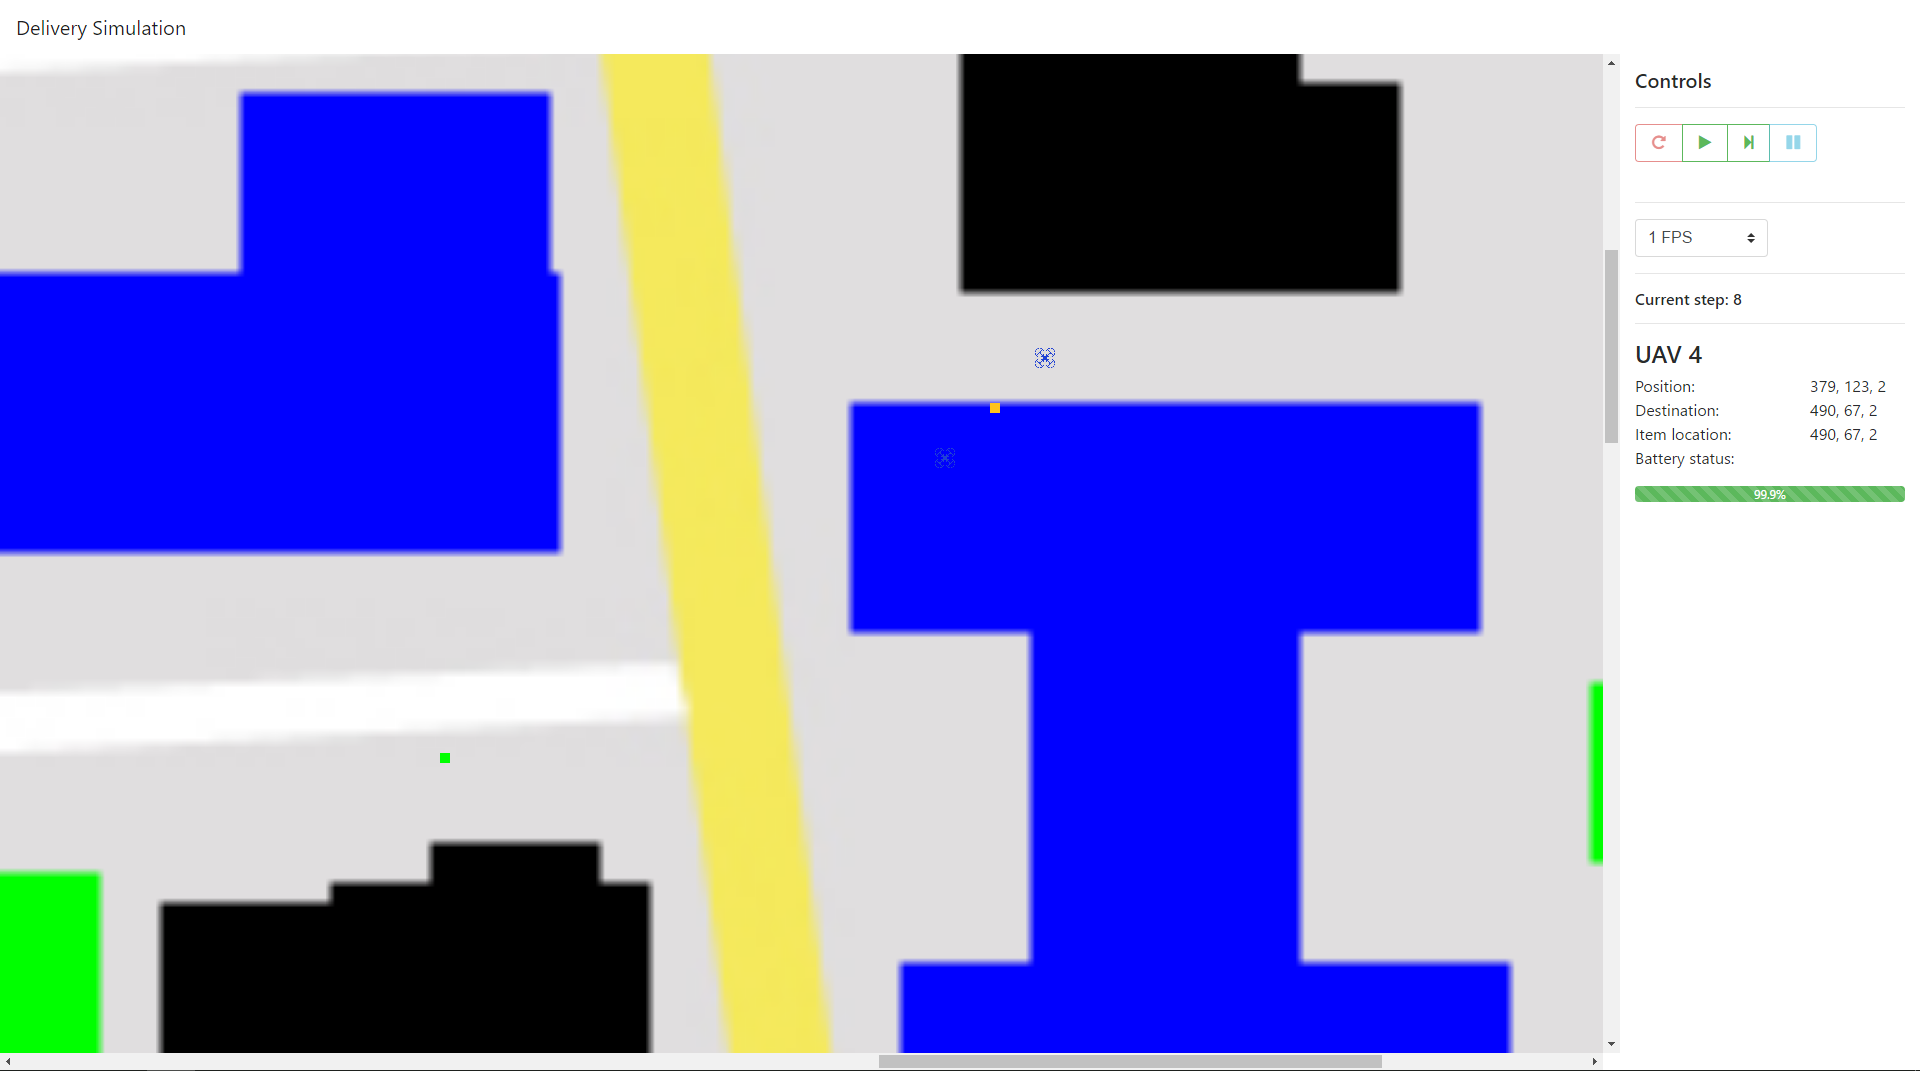
\includegraphics[width=\textwidth]{images/gui}
	\caption{The GUI of the simulation engine with UAV, Base-station (yellow),item destination (green) and detail of UAV (right)}
\end{figure}
The user interface consists of two parts: The file \textit{config.ini} to change the simulation scenario and a web server responsible for rendering the GUI and delivering it through a web browser. A GUI supports the ad-hoc analysis of the simulation before a big-enough number of steps has been reached to evaluate final results. Especially during the development of new algorithms, it is helpful to check if the UAVs behave as intended.\\
The configuration file is being parsed at the startup of the simulation engine and contains all the required settings for the simulation to work properly. It contains crucial information that have a high impact on an algorithm's performance and makes it easy to set up different scenarios, e.g. one might consider testing the results using different number of UAVs per depot or more or less depots itself.
Furthermore the impact of different battery capacity (in steps) can easily be simulated. A higher sensor range can be beneficial for an algorithm's performance but should be chosen realistically according to the model.\\
As mentioned earlier, the GUI is implemented using a web server. For the GUI to properly function, two image files are required. One contains the map as the user is supposed to see it. The other one stores information on obstacles and their respective heights using color codes. White means that there is no obstacle and other colors represent different altitude levels. An obstacle is any static object (such as trees or buildings etc.) that obstructs the movement of the UAV. The file will be parsed on start-up and the information stored in the model.  Depots are placed on obstacles, as close as possible to their intended center. For instance, on a 500x500 grid and a range of depots\footnote{Parameter "range of base station" in config.ini} of 250, the center is (250,250). If there is no obstacle on that position, the model will find the obstacle that is nearest to that location. Compare Figure 2 for an overview of the GUI.\\
The GUI allows for starting, pausing and resetting the simulation and shows the movement of UAVs in the space. It is implemented in a 2D fashion although internally the model calculates with 3-dimensional coordinates. The image's color codes for obstacles are used to represent the different altitudes. For now, the simulation tool supports 5 different height levels but one can easily modify the parser and define more colors for more altitude levels.
To be able to see more detailed information on each agent (UAV, base-station and item), one can click on the visual representation of the agent. The click activates a detail view. 

\subsection{Agents}\label{sec:UAV}
The most important agent of a UAV simulation is the UAV itself. We developed a realistic simulation representing the required components and behavior and omitted not required components to cover the delivery scenario. The simulated UAV has the following components:
	\begin{itemize}
			\item \textbf{Battery}: The battery has a limited battery life that decreases on each step. When the battery reaches a certain threshold (configurable), the UAV will fly to the nearest depot to recharge.
					\item \textbf{CargoBay:} The cargoBay represents the UAV's storage unit which can store one item.
		\item \textbf{FlightController:} This component contains the path-finding/route-planning algoritm. It represents a navigation unit. Multiple algorithms could be implemented, compare Section \ref{sec:algorithm} for an example. The algorithm uses the sensor to identify its neighboring fields at any step. Additionally it stores a perceived world which holds all fields that are already explored. The component can access all information from the other components and the UAV itself. On every step, the UAV calls the method "make\textunderscore step()" which has to be implemented in case of changing the algorithm.
		\item \textbf{CommunicationModule:} If the sensor found another UAV in the sensor's radius, this component will communicate with the other UAV and exchange grid information. Exchange of information on previously-unknown terrain helps when a UAV has to deliver an item to a new area of the map. This allows for precomputing optimal routes before exploring the actual area.
		\item \textbf{Sensor:} Scanning the grid for obstacles and other agents. This component is the interface to the model
	\end{itemize}

UAVs do not communicate with a central entity such as a control server organizing the flight traffic. They communicate with each other if they are in sensor range and only rely on their own sensor.
To optimize performance for the exchange of grids, the UAVs only store a dictionary containing their perceived world rather than a full matrix implemented in MESA's grid.
There is one dictionary for each altitude level, mapping coordinates to information whether there is an obstacle on that field or not.  
\\
The second agent in the simulation is the base-station. In the real world, this is the depot of a logistics company. It assigns orders to UAVs and hands items over to them. Depots are responsible for all items in a part of the map and for a subset of all drones. Also, they contain chargers for UAVs whose battery reached a low level. In the configuration, one can set how many depots are supposed to be on the map by specifying the number of fields the depot is responsible for (its delivery area). Depots are located as close to the center of their area as possible, but only on obstacles (on buildings). Items that are picked up from a depot can have different priorities in order to make the simulation more realistic. For example, items with high priority can be important and immediately required medical equipment or parcels for which a customer paid a higher fee to receive it faster.



\subsection{Analytics}\label{sec:KPI}
During a simulation run, data and results are being generated.
For evaluating the delivery scenario, we identified the following KPI's:
\begin{itemize}
	\item \textbf{Average walk length:} Describes the average number of steps taken for an item to be delivered. 
	\item \textbf{Average walk length divided by initial distance:} This data point is a ratio calculated by dividing the average number of steps taken by the initial distance from base-station to an item's destination. The initial distances are calculated as euclidean distances. Example: A value of 2 means that the average walk length is 2 times the initial distances.
	\item \textbf{Standard deviation of average walk lengths:} Represents the standard deviation of all walk lengths to get a better insight into the data additional to the average walk length.
	\item \textbf{Items delivered per UAV:} Items delivered divided by number of UAV's.
	\item \textbf{Average lifetime of item:} Calculation of the average lifetime of items by aggregating all item's lifetimes, divided by number of items. Lifetime is defined as the time from being available for delivery at the depot to the actual delivery at the item's destination.
\end{itemize}

The results are step-wise written out into a CSV file during the simulation and can for example be imported into a spreadsheet software or more sophisticated tools like R or any other application to run statistical analysis of the KPI's. Technically, this is realized by using MESA's DataCollector class. This allows for easy definition of values be calculated every step and export them to a CSV file. The KPI's can easily be extended or modified in the source code.

\section{Implementation of a sample algorithm: A Star}\label{sec:algorithm}
To determine the next move the UAV should make, the sensor is used to scan its surrounding cells. After the scan is done, the flight controller calculates the best possible cell. This calculation is done based on all known cells. Known, in this case, includes all cells that the UAV has either scanned or that it has exchanged with other UAVs. The best possible cell is the cell that minimizes the sum of the remaining distance to the destination of the UAV and the distance from the current position of the UAV to the cell the most. If the destination cell is already known to the UAV, the best possible cell would be that cell. If this is not the case, the best cell is only an approximation for the shortest path to the destination. When the best cell has been found, the shortest path from the current position of the UAV to the selected cell is calculated. To achieve this, the A* algorithm is used. A* was first described by Peter Hart, Nils J. Nilsson und Bertram Raphael \cite{hart.1968} and uses a heuristic function to search for the shortest path. In our case, this heuristic function is the remaining distance to the destination. Should there be no shortest path, for example if there is no known path to reach the best possible cell or the path is blocked by obstacles, then a new best cell is chosen and the previous one is excluded from this search.\\
This procedure is done every time the UAV needs to make a move. However, if the UAV already calculated the shortest path towards its destination, the calculation is skipped and the previously calculated shortest path is used instead. This can be done because there are no moving obstacles.\\
To avoid that a UAV gets stuck or that a UAV identifies a cell as the possible best cell multiple times, each visited cell is saved. Based on the number of times a cell was already visited, the calculated sum, determining the best cell, is weighted by the number of visits. By doing this, the UAV is not only less likely to get stuck, but also the exploration of unknown territory is promoted.

\section{Evaluation}\label{sec:evaluation}
The simulation engine presented in this paper allows for a convenient evaluation of a path planning algorithm in a 3-dimensional space. Also it helps to expose traditional algorithms to a swarm optimization problem as UAVs exchange their grid whenever they come close enough to each other.\\
A bottleneck is the calculation performance. On a mid-2015 Apple Macbook Pro with a i5 Dual core processor, the calculation of more than 10000 steps (run without GUI) still takes a very long time. Especially the scenario with 4 UAVs per base-station required many calculations over time due to more and more data to exchange. \\
The grid implementation of MESA is not performance-optimized. Also, the exchange of the grid is a complex task. It was tried to optimize performance by using dictionaries for the UAV's perceived world rather than storing a complete matrix. The model's internal grid also has been modified to just store numerical values for obstacles (1+ altitude), base-stations/depots (-1) or 0 for no content.\\
Still, we ran into a poor performance due to the algorithm itself and the inter-drone communication. The algorithm scanned the sensor area in every step although it already had the full knowledge required for calculating the best route.  \\
 \begin{table}[tbhp]\label{tab:results}
 	\centering

  \begin{tabular}{ | l | l | l |}
    \hline
     & \textbf{Scenario 1} 					& \textbf{Scenario 2}				\\ \hline
    Number of base-stations 	& \multicolumn{2}{|c|}{4}\\ \hline
    Number of UAVs 				& 8								& 16\\ \hline
    Steps simulated 				& \multicolumn{2}{|c|}{4x 10,000}\\ \hline
    Computation time 			& 12 hours 	each				& 24 hours each \\ \hline
    Average walk length 		& 106.75							& 102.35\\ \hline
    Average walk length divided by initial distance & 1.06 & 1.06 \\ \hline
    Standard deviation of average walk lengths & 60.71 & 62.22 \\ \hline 
    Items delivered 				& 267.75					&  569.75\\ \hline
    Items delivered per UAV & 33.47 & 35.61\\ \hline
    Average lifetime of items &3211.58 & 2994.49 \\ \hline
    \hline
  \end{tabular}
	 	
  \caption{Results of two simulation scenarios}
 \end{table}
We ran two simulation scenarios, both with 4 depots (=base-stations) and 8 and 16 UAVs, respectively. The map had a size of 500x500x4 fields (4 altitude levels). Every scenario was run four times with 10000 steps each, in order to create meaningful results. The results are mean values of the KPIs over the four runs. Compare table 1 for the results. The average walk length converged converged at around 102-106 steps, for both scenarios. But we ran into a quite high standard deviation of around 60 steps. Unsurprisingly, in Scenario 1, less items were delivered compared to scenario 2. Interestingly, the average number of steps divided by the euclidean (direct) distance almost reached 1. Unfortunately, we did not measure the standard deviation for this value. Due to the high standard deviation of the average walk length, we also suppose a very high one here. It seems the exploration phase ended quite early, after around 2500 steps for scenario two (compare Figure 3), considering that every UAV had to move in an area of 62,500 field (125x125x4 fields) and explore it before being able to compute best routes for all fields. The average lifetime of items reached very high values, most likely due to the fact that depots always hold more items (5) than delivery UAVs available (2 or 4 per depot). The inter-UAV communication most likely is a strong reason for this early convergence. The quite good values for average walk length probably also lie in the nature of the simulated map. Most obstacles have a height of less than 4 (maximum) and thus UAVs just passed over them. \\
 
 \begin{figure}\label{fig:eval}
 \centering
 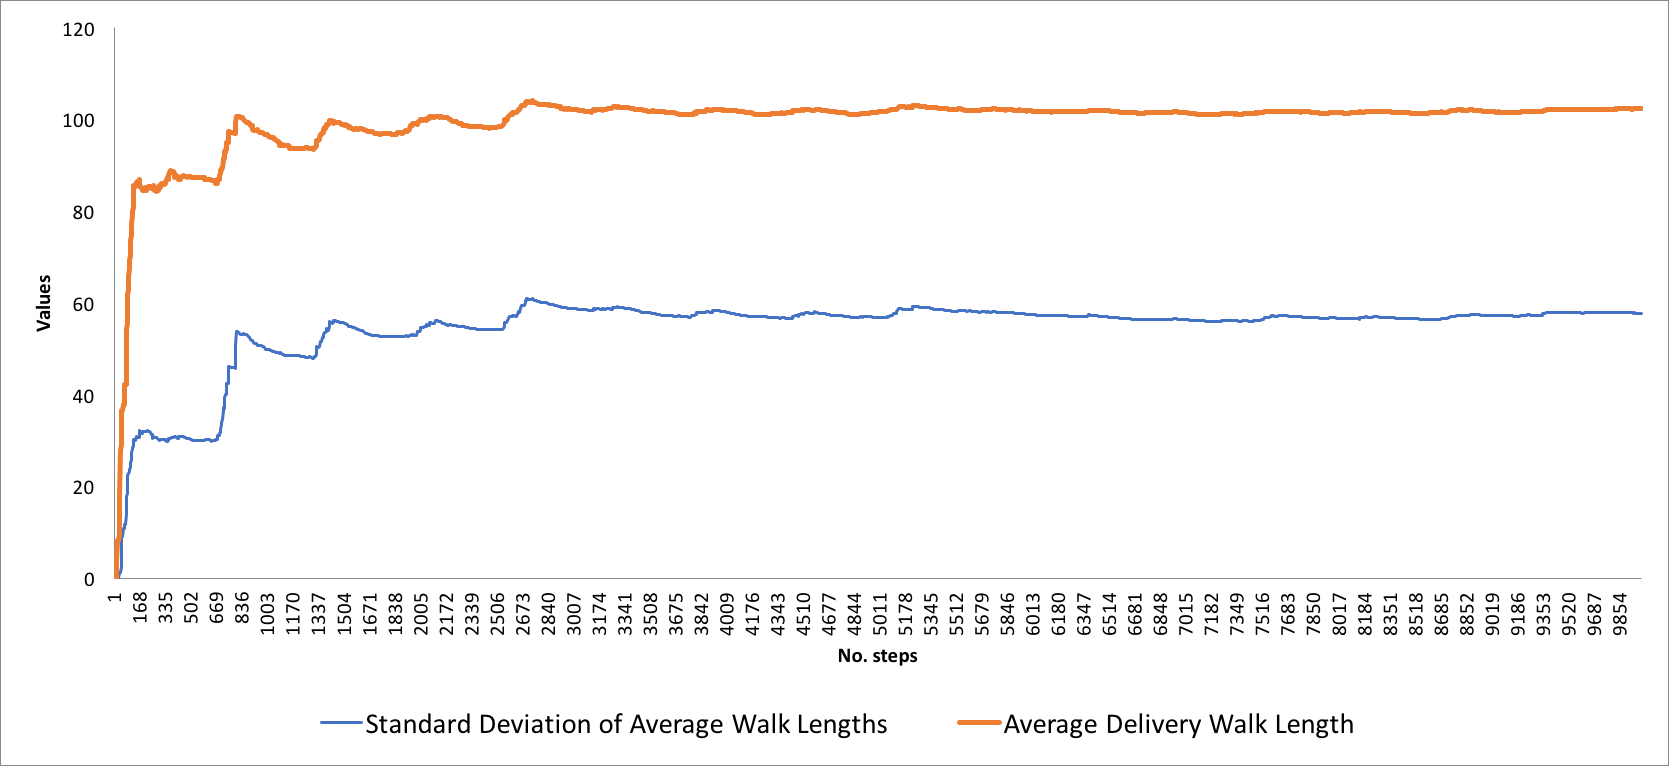
\includegraphics[width=\textwidth]{images/graph}
 \caption{Plot of average walk length and standard deviation of scenario 2}
 \end{figure}

\section{Conclusion}\label{sec:conclusion}
This paper presented a new simulation engine specifically developed for the delivery use-case with autonomous UAV not being controlled by a central control server. Delivery of items will be relevant in the near future and a simulation engine is required to test for different algorithms and management systems, such as different numbers of depots or rural against urban regions. The engine supports multiple depots and UAVs, communication between UAV and different altitude levels for testing. It is based on the MESA modeling framework whereas many adjustments for performance have been implemented. The GUI allows for visual evaluation of the simulation's progress and the CSV output helps analyzing the final scenario results. The simulation of a battery helps to understand how far a destination should be from a depot and thus how many depots are required. \\
The example implementation using the A* star algorithm showed that there is still space for optimization, especially finding criteria when the UAVs should actually stop exchanging their grid. Also, more precise KPI's should be defined and implemented.\\
The scenario described here does not simulate the parcels being delivered to the depots, it just simulates the "last mile" from the depot to the customer. Thus, the scenario could be modified by having UAVs transporting items from a main depot to smaller, final delivery units. From these, the actual delivery UAVs could transport goods to the customers. Such a simulation allows to test for the feasibility of taking the intermediate transportation of goods from the street to the air. The application might also be modified to make use of scouting UAVs that explore the area and only them sharing the grid information with the delivery UAVs. This approach could reduce the amount of inter-UAV communication. Moving obstacles will be implemented in the future as well.


\bibliographystyle{scsproc}
% AUTHOR: Include your bib file here
\bibliography{paper}

\section*{Author Biographies}

\textbf{\uppercase{Jan Gerald Huenges}} is a master student of Management Information Systems at TU Berlin. He concentrates on software engineering and  ... His email address is \email{wsc15roeder@gmail.com}.

\textbf{\uppercase{Aleksandra Pranskaityte}} is a master student of Management Information Systems at TU Berlin.  Her email address is \email{wsc16frazier@gmail.com}.

\textbf{\uppercase{Santiago Masip Gimeno}}, Technical Engineer in Administrative Data Processing at Polytechnic University of Valencia. Management Information Systems student at TU Berlin focuses his studies on Data Analytics field.  His email address is \email{masipgimeno@campus.tu-berlin.de}.

\textbf{\uppercase{Dominik Schroeck}} is a master student of Management Information Systems at TU Berlin. He received the bachelor's degree at Paderborn University, focussing on O.R. and decision support. He has a strong interest in quantitative research and automation in financial services. His email address is \email{dominik.schroeck@campus.tu-berlin.de}.

\uppercase{M.Sc. \textbf{Christopher-Eyk Hrabia}} received a degree in computer science from the Technische Universität Berlin (TUB) in 2012. At the DAI-Lab of TUB he researches in the field of multi-agent and multi-robot system with a focus on high-level control of autonomous, adaptive and self-organizing unmanned aerial vehicles. \email{christopher-eyk.hrabia@dai-labor.de}.

\uppercase{Prof. Dr.-Ing. Habil. \textbf{Sahin Albayrak}} is the head of the chair Agent Technologies in Business
Applications and Telecommunication. He is the founder and head of the DAI-Lab, currently employing about one hundred researchers and support staff. His email address is \email{sahin.albayrak@dai-labor.de}.

%\newpage
%
%\begin{figure*}[htb]
%{
%\centering
%First Name Last Name 1 \\
%First Name Last Name 2 \\
%\vspace{12pt}
%Affiliation \\
%Address, City, Country \\
%E-mail address
%\caption{Example title page heading with 2 authors from the same institution.\label{fig2same}}
%}
%\end{figure*}
%
%\begin{figure*}[htb]
%{
%\centering
%\begin{tabular}{ccc}
%\phantom{Entries to adjust spacing - ignore} & \phantom{intermediate space} & \phantom{Entries to adjust spacing - ignore} \\
%First Name Last Name 1 & & First Name Last Name 2 \\
%\\
%Affiliation 1 & & Affiliation 2 \\
%Address, City, Country 1 & & Address, City, Country 1 \\
%E-mail address 2 & & E-mail address 2 
%\end{tabular}
%\caption{Example title page heading with 2 authors from different institutions.\label{fig2different}}
%}
%\end{figure*}
%
%\begin{figure*}[htb]
%{
%\centering
%\begin{tabular}{ccc}
%\phantom{This adjusts spacing - ignore} & \phantom{This adjusts spacing - ignore} & \phantom{This adjusts spacing - ignore} \\
%First Name Last Name 1 & & First Name Last Name 2 \\
%\\
%Affiliation 1 & & Affiliation 2 \\
%Address, City, Country 1 & & Address, City, Country 1 \\
%E-mail address 2 & & E-mail address 2 \\
%\\
%\\
%& First Name Last Name 3 \\
%\\
%& Affiliation 3\\
%& Address, City, Country \\
%& E-mail address 2 
%\end{tabular}
%\caption{Alternate example title page heading with 3 authors from different institutions. \label{fig3different}}
%}
%\end{figure*}
%
%\begin{figure*}[htb]
%{
%\centering
%\begin{tabular}{ccc}
%\phantom{Adjust spacing using these entries} & \phantom{intermediate space} & \phantom{Adjust spacing using these entries} \\
%First Name Last Name 1 & & First Name Last Name 2 \\
%\\
%Affiliation 1 & & Affiliation 2 \\
%Address, City, Country 1 & & Address, City, Country 1 \\
%E-mail address 2 & & E-mail address 2 \\
%\\ \\
%First Name Last Name 3 & & First Name Last Name 4 \\
%\\
%Affiliation 3 & & Affiliation 4 \\
%Address, City, Country 1 & & Address, City, Country 1 \\
%E-mail address 2 & & E-mail address 2 
%\end{tabular}
%\caption{Example title page heading with 4 authors from different institutions.\label{fig4different}}
%}
%\end{figure*}
%
\end{document}
